\documentclass[11pt,a4paper,titlepage,oneside]{report}
\usepackage{titling}
\usepackage{graphicx}
\usepackage{mathtools}
\usepackage{lmodern}
\usepackage{amsmath}
\usepackage{float}
\usepackage{subfig}
\usepackage{listings}
\usepackage[hidelinks]{hyperref}

%% Memoir layout setup

%% NOTE: You are strongly advised not to change any of them unless you
%% know what you are doing.  These settings strongly interact in the
%% final look of the document.

% Dependencies
\usepackage{bfhlogo}
\usepackage{etoolbox}% http://ctan.org/pkg/etoolbox

\makeatletter
%%begin novalidate
%% Titlepage adjustments
\pretitle{\vspace{0pt plus 0.7fill}\begin{center}\Huge}
\posttitle{\end{center}\par}
\preauthor{\par\begin{center}\let\and\\\Large}
\postauthor{\end{center}}
\predate{\par\begin{center}\Large}
\postdate{\end{center}}
%%end novalidate
\def\@advisors{}
\newcommand{\advisors}[1]{\def\@advisors{#1}}
\def\@department{}
\newcommand{\department}[1]{\def\@department{#1}}
\def\@thesistype{}
\newcommand{\thesistype}[1]{\def\@thesistype{#1}}

\renewcommand{\maketitlehooka}{\noindent\bfhlogo[2cm]}

\renewcommand{\maketitlehookb}{\vspace{1in}%
  \par\begin{center}\Large\sffamily\@thesistype\end{center}}

\renewcommand{\maketitlehookd}{%
  \vfill\par
  \begin{flushright}
    \sffamily
    \@advisors\par
    \@department, BFH
  \end{flushright}
}

% Fix the chapters (unnecessary space)
\patchcmd{\@makechapterhead}{\vspace*{50\p@}}{}{}{}% Removes space above \chapter head
\patchcmd{\@makeschapterhead}{\vspace*{50\p@}}{}{}{}% Removes space above \chapter* head

\makeatother

\setlength{\droptitle}{-48pt}


\setlength{\parindent}{0pt}

\title{ORB Slam Point Cloud generation on Apalis iMX8}
\author{Stefan Eichenberger}
\date{February 2019}
\advisors{Marcus Hudritsch}
\department{TSM CPVR Lab}

\lstset{
	basicstyle=\ttfamily\scriptsize
}

\begin{document}
\title{Open source SLAM library for embedded systems}

\maketitle
\begin{abstract}
  Simultaneous location and mapping (SLAM) is a technology used for robot navigation and augmented reality. Today most SLAM libraries are either proprietary or not meant for embedded systems. In this thesis we write a library which is open source and achieves frame rates of above 30 fps when running on embedded devices.
\end{abstract}

\tableofcontents

\chapter{Planing}

This chapter describes the planing of the master thesis. The first section lists the requirements the second section shows the time planing.

\section{Requirement Specification}

This section lists the features that must and shall be implemented during the master thesis. The word must means that these are hard requirements. Shall describes nice to have features that aren't hardly required. Can are options that are not required at all. The numbers after \# are IDs found in the Gantt chart of figure \ref{fig:gantt}.

\subsection{SLAM Library \#42}
A SLAM library must be written which runs at 30 fps on stereo gray scale images at a resolution of 640x480 on two Intel i5-7Y54 CPUs.
\subsubsection{SVO based algorithm \#44}
A first implementation of the library shall be based on SVO. However, it's not mandatory to be the exact SVO algorithm.
\subsubsection{Plane Detection \#45}
The library must provide a mechanism to detect points laying on a plane and to remove redundant points.
\subsubsection{Mesh Creation \#46}
The library must create a mesh from the sparse point cloud. The mesh shall contain textures from corresponding images.
\subsubsection{IMU Integration \#47}
The library must provide an interface to feed data from an IMU to estimate the motion model.
\subsubsection{Relocation \#48}
The library shall provide an interface to find the current location of the camera based on a pre-generated map
\subsubsection{Language}
The library must provide a Python 3 interface.
\subsubsection{CPU}
The library must run on x86/amd64 but shall not be limited to this architecture.
\subsection{OpenCL}
OpenCL can be used to increase the performance of the library
\subsection{Example Application \#43}
An application must be written that shows the capabilities of the library. 
\subsubsection{Mapping}
The application must create a sparse map of a typical room with four walls, one door and two windows. However, it shall not be limited to such an environment.
\subsubsection{Exporting}
The application shall have a feature to export a generated map for further use.
\subsubsection{Relocation}
The application shall have a mechanism to load a pre-generated map that can be used to do relocation.

\section{Planning}
The master thesis is honored with 27 ECTS. 1 ECTS consumes 25-30h which results in a total of 675-810h. Assuming the lower effort and 8 working hours per day, we have to spend 84.375 working days. Because the thesis is done part time a full year can be used. We assume one year has 48 weeks. During the first 16 weeks only 1.5 days can be used for the master thesis (because of additional modules). This means during the first 16 weeks we only work 24 days on the project. 60.375 days are left for the last 32 weeks. This results in 1.89 days work during the 32 weeks. This leaves room for vacation and problems. Figure \ref{fig:gantt} shows the initial planing. The first implementation of the algorithm takes much longer than the rest because only 1.5 days can be spent for the thesis during this period.

\begin{figure}[H]
	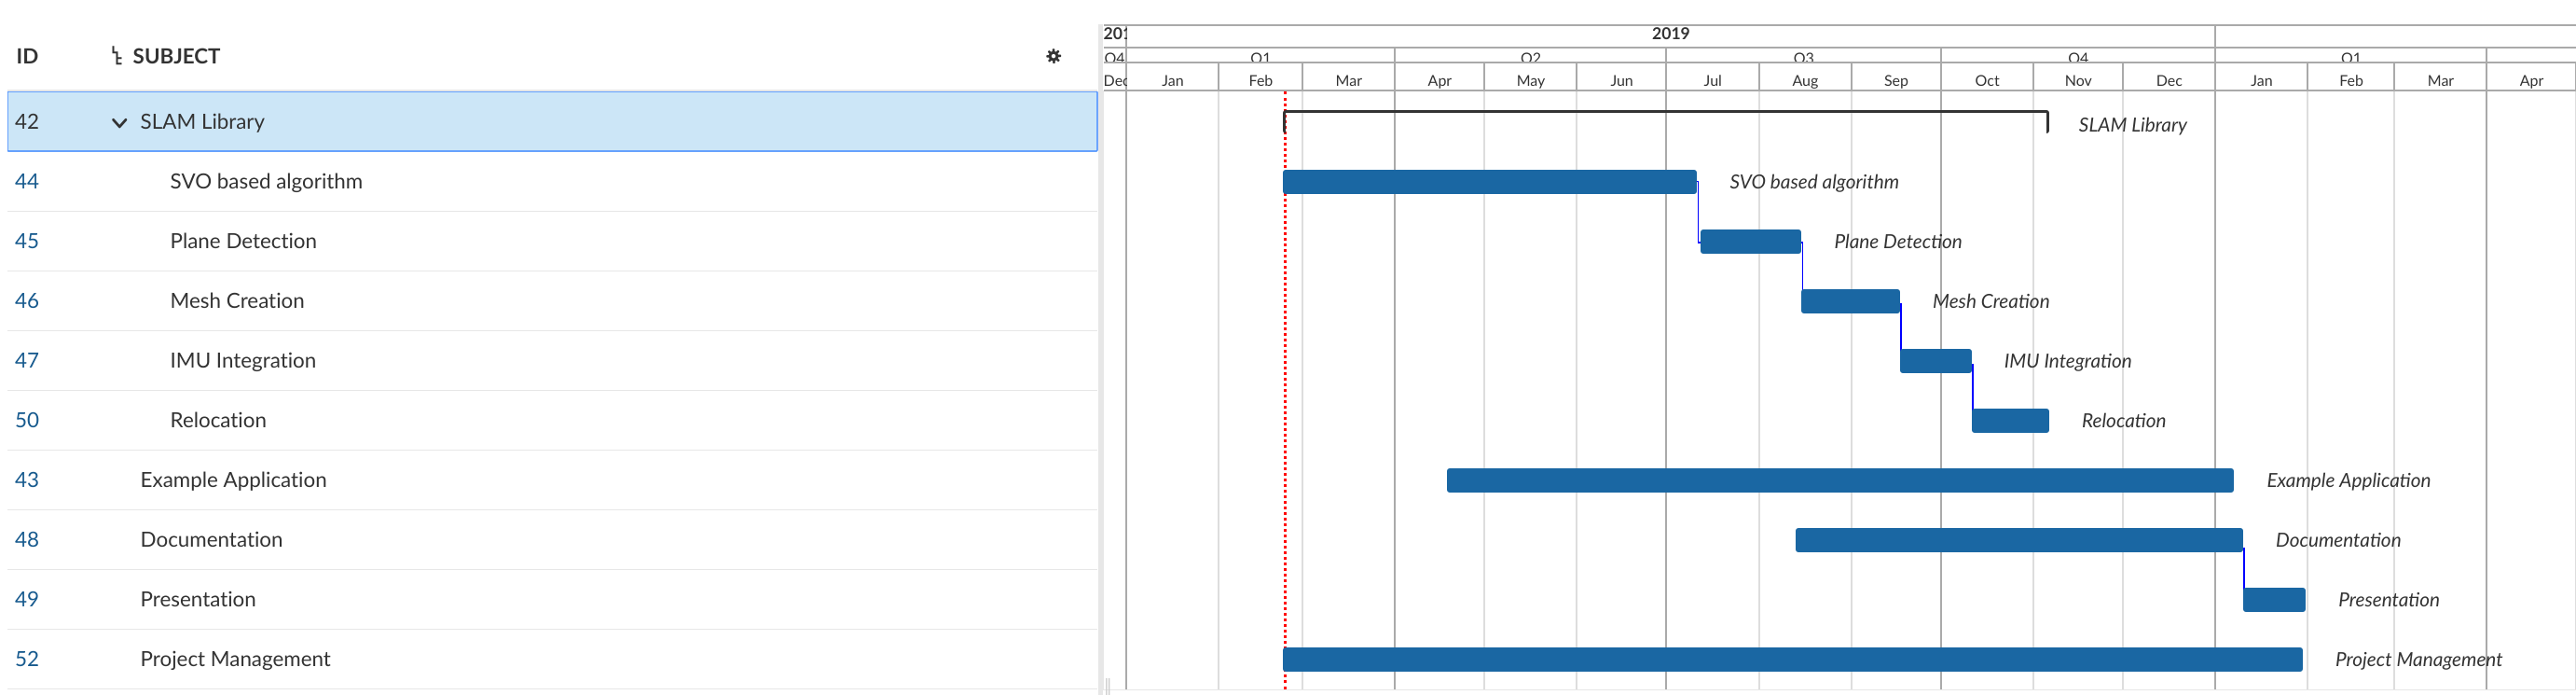
\includegraphics[width=1.0\textwidth]{img/gantt.png}
	\caption{Initial planing}\label{fig:gantt}
\end{figure}

\end{document}
